\documentclass[utf8x, 12pt]{G7-32}

% Настройки стиля ГОСТ 7-32
% Для начала определяем, хотим мы или нет, чтобы рисунки и таблицы нумеровались в пределах раздела, или нам нужна сквозная нумерация.
\EqInChapter % формулы будут нумероваться в пределах раздела
\TableInChapter % таблицы будут нумероваться в пределах раздела
\PicInChapter % рисунки будут нумероваться в пределах раздела
\usepackage{slashbox}

\usepackage[table,xcdraw]{xcolor}

% Добавляем гипертекстовое оглавление в PDF
\usepackage[
bookmarks=true, colorlinks=true, unicode=true,
urlcolor=black,linkcolor=black, anchorcolor=black,
citecolor=black, menucolor=black, filecolor=black,
]{hyperref}

% Изменение начертания шрифта --- после чего выглядит таймсоподобно.
% \usepackage{cyrtimespatched}

% графика
\usepackage{graphicx}
\graphicspath{ {./img/} }

% отделять первую строку раздела абзацным отступом
\usepackage{indentfirst} 

% Пакет Tikz
\usepackage{tikz}
\usetikzlibrary{arrows,positioning,shadows}

% Произвольная нумерация списков.
\usepackage{enumerate}

% ячейки в несколько строчек
\usepackage{multirow}

% itemize внутри tabular
\usepackage{paralist,array}

% объявляем новую команду для переноса строки внутри ячейки таблицы
\newcommand{\specialcell}[2][c]{%
	\begin{tabular}[#1]{@{}c@{}}#2\end{tabular}}

\usepackage{tikz}
\usepackage{pgfplots}
\usepackage{pdfpages}
\usepackage{caption}
\usepackage{longtable}
% \captionsetup[table]{position=top}
% Листинги

\usepackage{listings}
\usepackage{caption}

\usepackage{courier}
\usepackage{wrapfig}

\usepackage{xcolor}
\captionsetup[lstlisting]{singlelinecheck=off, justification=raggedright}


\definecolor{codegreen}{rgb}{0,0.6,0}
\definecolor{codegray}{rgb}{0.5,0.5,0.5}
\definecolor{codepurple}{rgb}{0.58,0,0.82}
\definecolor{backcolour}{rgb}{0.95,0.95,0.92}


% Значения по умолчанию
\lstset{
  % подсветка синтаксиса
  backgroundcolor=\color{backcolour},   
  commentstyle=\color{codegreen},
  keywordstyle=\color{magenta},
  numberstyle=\tiny\color{codegray},
  stringstyle=\color{codepurple},
  basicstyle= \footnotesize,
  breakatwhitespace=true,% разрыв строк только на whitespacce
  breaklines=true,       % переносить длинные строки
%   captionpos=b,          % подписи снизу -- вроде не надо
  inputencoding=koi8-r,
  numbers=left,          % нумерация слева
  numberstyle=\footnotesize,
  showspaces=false,      % показывать пробелы подчеркиваниями -- идиотизм 70-х годов
  showstringspaces=false,
  showtabs=false,        % и табы тоже
  stepnumber=1,
  tabsize=4,              % кому нужны табы по 8 символов?
  frame=single,
  escapeinside={(*}{*)}, %выделение
  literate={а}{{\selectfont\char224}}1
  {б}{{\selectfont\char225}}1
  {в}{{\selectfont\char226}}1
  {г}{{\selectfont\char227}}1
  {д}{{\selectfont\char228}}1
  {е}{{\selectfont\char229}}1
  {ё}{{\"e}}1
  {ж}{{\selectfont\char230}}1
  {з}{{\selectfont\char231}}1
  {и}{{\selectfont\char232}}1
  {й}{{\selectfont\char233}}1
  {к}{{\selectfont\char234}}1
  {л}{{\selectfont\char235}}1
  {м}{{\selectfont\char236}}1
  {н}{{\selectfont\char237}}1
  {о}{{\selectfont\char238}}1
  {п}{{\selectfont\char239}}1
  {р}{{\selectfont\char240}}1
  {с}{{\selectfont\char241}}1
  {т}{{\selectfont\char242}}1
  {у}{{\selectfont\char243}}1
  {ф}{{\selectfont\char244}}1
  {х}{{\selectfont\char245}}1
  {ц}{{\selectfont\char246}}1
  {ч}{{\selectfont\char247}}1
  {ш}{{\selectfont\char248}}1
  {щ}{{\selectfont\char249}}1
  {ъ}{{\selectfont\char250}}1
  {ы}{{\selectfont\char251}}1
  {ь}{{\selectfont\char252}}1
  {э}{{\selectfont\char253}}1
  {ю}{{\selectfont\char254}}1
  {я}{{\selectfont\char255}}1
  {А}{{\selectfont\char192}}1
  {Б}{{\selectfont\char193}}1
  {В}{{\selectfont\char194}}1
  {Г}{{\selectfont\char195}}1
  {Д}{{\selectfont\char196}}1
  {Е}{{\selectfont\char197}}1
  {Ё}{{\"E}}1
  {Ж}{{\selectfont\char198}}1
  {З}{{\selectfont\char199}}1
  {И}{{\selectfont\char200}}1
  {Й}{{\selectfont\char201}}1
  {К}{{\selectfont\char202}}1
  {Л}{{\selectfont\char203}}1
  {М}{{\selectfont\char204}}1
  {Н}{{\selectfont\char205}}1
  {О}{{\selectfont\char206}}1
  {П}{{\selectfont\char207}}1
  {Р}{{\selectfont\char208}}1
  {С}{{\selectfont\char209}}1
  {Т}{{\selectfont\char210}}1
  {У}{{\selectfont\char211}}1
  {Ф}{{\selectfont\char212}}1
  {Х}{{\selectfont\char213}}1
  {Ц}{{\selectfont\char214}}1
  {Ч}{{\selectfont\char215}}1
  {Ш}{{\selectfont\char216}}1
  {Щ}{{\selectfont\char217}}1
  {Ъ}{{\selectfont\char218}}1
  {Ы}{{\selectfont\char219}}1
  {Ь}{{\selectfont\char220}}1
  {Э}{{\selectfont\char221}}1
  {Ю}{{\selectfont\char222}}1
  {Я}{{\selectfont\char223}}1
}

\lstloadlanguages{
  C++
}

% Стиль для псевдокода: строчки обычно короткие, поэтому размер шрифта побольше
\lstdefinestyle{pseudocode}{
  basicstyle=\small,
  keywordstyle=\color{black}\bfseries\underbar,
  language=Pseudocode,
  numberstyle=\footnotesize,
  commentstyle=\footnotesize\it
}

% Стиль для обычного кода: маленький шрифт
\lstdefinestyle{realcode}{
  basicstyle=\scriptsize,
  numberstyle=\footnotesize
}

% Стиль для коротких кусков обычного кода: средний шрифт
\lstdefinestyle{simplecode}{
  basicstyle=\footnotesize,
  numberstyle=\footnotesize
}

% Стиль для BNF
\lstdefinestyle{grammar}{
  basicstyle=\footnotesize,
  numberstyle=\footnotesize,
  stringstyle=\bfseries\ttfamily,
  language=BNF
}

% Определим свой язык для написания псевдокодов на основе Python
\lstdefinelanguage[]{Pseudocode}[]{Python}{
  morekeywords={each,empty,wait,do},% ключевые слова добавлять сюда
  morecomment=[s]{\{}{\}},% комменты {а-ля Pascal} смотрятся нагляднее
  literate=% а сюда добавлять операторы, которые хотите отображать как мат. символы
    {->}{\ensuremath{$\rightarrow$}~}2%
    {<-}{\ensuremath{$\leftarrow$}~}2%
    {:=}{\ensuremath{$\leftarrow$}~}2%
    {<--}{\ensuremath{$\Longleftarrow$}~}2%
}[keywords,comments]

% Свой язык для задания грамматик в BNF
\lstdefinelanguage[]{BNF}[]{}{
  morekeywords={},
  morecomment=[s]{@}{@},
  morestring=[b]",%
  literate=%
    {->}{\ensuremath{$\rightarrow$}~}2%
    {*}{\ensuremath{$^*$}~}2%
    {+}{\ensuremath{$^+$}~}2%
    {|}{\ensuremath{$|$}~}2%
}[keywords,comments,strings]

% Подписи к листингам на русском языке.
\renewcommand\lstlistingname{\cyr\CYRL\cyri\cyrs\cyrt\cyri\cyrn\cyrg}
\renewcommand\lstlistlistingname{\cyr\CYRL\cyri\cyrs\cyrt\cyri\cyrn\cyrg\cyri}



\begin{document}

\frontmatter % выключает нумерацию ВСЕГО; здесь начинаются ненумерованные главы: реферат, введение, глоссарий, сокращения и прочее.

\begin{table}[ht]
	\centering
	\begin{tabular}{|c|p{400pt}|} 
	\hline
		\begin{tabular}[c]{@{}c@{}} 
\includegraphics[scale=0.37]{EmblemBMSTU} \\\end{tabular} &
		\footnotesize\begin{tabular}[c]{@{}c@{}}\textbf{Министерство~науки~и~высшего~образования~Российской~Федерации}\\\textbf{Федеральное~государственное~бюджетное~образовательное~учреждение}\\\textbf{~высшего~образования}\\\textbf{«Московский~государственный~технический~университет}\\\textbf{имени~Н.Э.~Баумана}\\\textbf{(национальный~исследовательский~университет)»}\\\textbf{(МГТУ~им.~Н.Э.~Баумана)}\\\end{tabular}  \\
	\hline
	\end{tabular}
\end{table}
\noindent\rule{\textwidth}{4pt}
\noindent\rule[14pt]{\textwidth}{1pt}
\hfill 
\noindent
\makebox{ФАКУЛЬТЕТ~}%
\makebox[\textwidth][l]{\underline{~~~~«Информатика и системы управления»~~~~~~~~~~~~~~~~~~~~~~~~~~~~~~~~~~~~~~~~~~~~}}%
\\
\noindent
\makebox{КАФЕДРА~}%
\makebox[\textwidth][l]{\underline{~~~~~~~«Программное обеспечение ЭВМ и информационные технологии»~~~~~~~~}}%
\\


\begin{center}
	\vspace{3cm}
	{\bf\huge Отчёт\par}
	{\bf\Large по лабораторной работе № 5\par}
	\vspace{0.5cm}
\end{center}


\noindent
\makebox{\large{\bf Название:}~~~}
\makebox[\textwidth][l]{\large\underline{~Многопоточная реализация конвейера~~~~~~~~~~~~~}}\\

\noindent
\makebox{\large{\bf Дисциплина:}~~~}
\makebox[\textwidth][l]{\large\underline{~Анализ алгоритмов~~~~~~~~~~~~~~~~~~~~~~~~~~~~~~~~~~~~~~~~~~~~~~~~~~~~}}\\

\vspace{1.5cm}
\noindent
\begin{tabular}{l c c c c c}
    Студент      & ~ИУ7-55Б~               & \hspace{3.5cm} & \hspace{3.5cm}                 & &  И. Е. Афимин \\\cline{2-2}\cline{4-4} \cline{6-6} 
    \hspace{3cm} & {\footnotesize(Группа)} &                & {\footnotesize(Подпись, дата)} & & {\footnotesize(И.О. Фамилия)}
\end{tabular}

\vspace{1cm}

\noindent
\begin{tabular}{l c c c c}
    Преподователь & \hspace{6cm}   & \hspace{3.5cm}                 & & Л.Л. Волкова \\\cline{3-3} \cline{5-5} 
    \hspace{3cm}  &                & {\footnotesize(Подпись, дата)} & & {\footnotesize(И.О. Фамилия)}
\end{tabular}

\begin{center}	
	\vfill
	\large \textit {Москва, 2020}
\end{center}

\thispagestyle {empty}
\pagebreak

\tableofcontents
\pagebreak

\Introduction
    Муравьиный алгоритм -- один из эффективных
    полиномиальных алгоритмов для нахождения 
    приближённых решений задачи коммивояжёра, 
    а также решения аналогичных задач поиска маршрутов на графах.
        
    Целью данной лабораторной работы является
    изучение муравьиных алгоритмов и приобретение
    навыков параметризации методов на примере
    муравьиного алгоритма, примененного к задаче коммивояжера.
        
    Задачи данной лабораторной работы:
    \begin{enumerate}
        \item рассмотренть муравьиный алгоритм и алгоритм полного перебора в задаче коммивояжера;
        \item реализовать эти алгоритмы;
        \item сравнить время работы этих алгоритмов.
    \end{enumerate}

\newpage

\mainmatter % это включает нумерацию глав и секций в документе ниже

\chapter{ Аналитический раздел}
\label{cha:analytical}
    В данном разделе будут рассмотрены 
    алгоритмы поиска слов в слове.

    \section{Алгоритм полного перебора}
        Алгоритм полного перебора -- это алгоритм разрешения математических задач,
        который можно отнести к классу способов нахождения решения рассмотрением
        всех возможных вариантов. 
        Полный перебор (или метод «грубой силы», англ. brute force) -- метод решения математических задач.
        Относится к классу методов поиска решения исчерпыванием всевозможных вариантов.
        Сложность полного перебора зависит от количества всех возможных решений задачи.
        Если пространство решений очень велико, то полный перебор может не дать результатов 
        в течение нескольких лет или даже столетий.
        
        В данном случае следует перебирать слова в словаре, 
        пока не встретится нужное слово, 
        следовательно, время работы оценивается как $ O(n)$.

    \section{Алгоритм двоичного поиска}
        Целочисленный двоичный поиск (бинарный поиск) (англ. binary search) -- алгоритм поиска
        объекта по заданному признаку в множестве объектов, упорядоченных по тому же самому признаку,
        работающий за логарифмическое время. 

        Принцип двоичный поиска заключается в том, 
        что на каждом шаге множество объектов делится на две части 
        и в работе остаётся та часть множества, 
        где может находится искомый объект. 
        В зависимости от постановки задачи,
        процесс может остановливается, 
        когда получен первый или же последний индекс вхождения элемента.
        Последнее условие -- это левосторонний/правосторонний двоичный поиск. 

    \section{Алгоритм поиска по сегментам}
        Суть данного алгоритма заключается в том,
        что необходимо разбить словарь на сегменты.
        Каждый сегмент определяет первую букву слов,
        которые находятся в нем. 
        Для того, чтобы найти слово в таком
        словаре необходимо определить сегмент, где может находиться слово,
        а после произвести поиск в данном сегменте.

\newpage
\chapter{ Конструкторский раздел}
\label{cha:design}
        В данном разделе будут рассмотрены описание системы, требования к функциональности ПО
        и определены способы тестирования.
    \section{Описание системы}
        Система состоит из трех этапов (рисунок \ref{schema:conveyor}),
        который последовательно соединены между собой. 
        Каждый этап выполняет возведение в квадрат
        полученного на вход элемента. 
        Для уменьшения влияния времени диспетчеризации 
        будет вызываться системный вызов sleep 
        с разным временем ожидания для каждого этапа.
        Время попадания в каждую очередь логируется.

    \begin{figure}[h!]
        \centering
            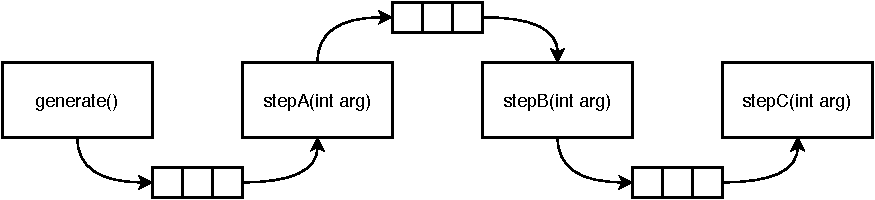
\includegraphics[scale=0.9]{schema_conveyor.pdf}
            \caption{Схема конвейерной обработки}
            \label{schema:conveyor}
    \end{figure}


    \section{Требования к функциональности ПО}
        В данной работе требуется обеспечить следующую минимальную функциональность консольного приложения:
        \begin{enumerate}
            \item предоставить возможность ввода количества генерируемых элементов в системе;
            \item обеспечить вывод времени получения и отправки элемента конвейера.
        \end{enumerate}

    \section{Тесты}
        Тестирование ПО будет проводиться методом чёрного ящика. 
        Эффект от конвейеризации становиться заметен,
        если время выполнения этапа много больше времени диспетчеризации. 
        Каждый этап будет возводить число в квадрат и вызывать системный вызов sleep 
        с разным временем ожидания для каждого этапа.

    \section{Вывод}
        В данном разделе были рассмотрены схема алгоритмов 
        обработки элементов линии конвейера и
        описаны требования к функциональности ПО.
        

\newpage
\chapter{ Технологический раздел}
\label{cha:technological}

    В данном разделе будут выбраны средства реализации ПО и представлен листинг кода. 

    \section{Средства реализации}
        В данной работе используется язык программирования python \cite{c-sharp}, так как
        он позволяет написать программу в относительно малый срок.
        В качестве среды разработки использовался Jupyter Notebook.

        Для замера процессорного времени была использована функция process\_time модуля time.
        Она возвращает значение в долях секунды суммы системного и пользовательского процессорного времени текущего процесса и 
        не включает время, прошедшее во время сна.

    \section{Листинг программы}
        Ниже представлены листинги кода алгоритмов поиска слова в словаре:
        \begin{enumerate}
            \item полным перебором (листинг \ref{lst:brute-force});
            \item бинарным поиском (листинг \ref{lst:binary});
            \item поиском по сегментам (листинг \ref{lst:segment}).
        \end{enumerate}
        
        \begin{lstlisting}[language=python, label=lst:brute-force, caption=Реализация алгоритма поиска слов в словаре полным перебором]
class BruteForceDictionary:
    "Словарь с поиском ключа перебором"
    def __init__(self):
        self.data = []
    
    def keys(self):
        return list(self.__iter__())

    def __getitem__(self, key : str) -> int:
        i = self.__get_index_key(key)
        if i > -1:
            return self.data[i][1]
        return None

    def __setitem__(self, key: str, value: int):
        i = self.__get_index_key(key)
        if i < 0:
            self.data.append((key, value))
        else:
            self.data[i] = (key, value)

    def __contains__(self, key: str):
        return self.__get_index_key(key) > -1

    def __iter__(self):
        return iter(map(lambda pair: pair[0], self.data))

    def __get_index_key(self, key: str) -> int:
        i = 0
        for i, pair in enumerate(self.data):
            if pair[0] == key:
                return i
        return -i - 1
        \end{lstlisting}

        \begin{lstlisting}[language=python, label=lst:binary, caption=Реализация алгоритма двоичного поиска слова в словаре]
class BinarySearchDictionary:
    "Словарь с двоичным поиском ключа"
    def __init__(self):
        self.data = []
        self.n = 0

    def keys(self):
        return list(self.__iter__())

    def __getitem__(self, key : str) -> int:
        i = self.__get_index_key(key)
        if i >= 0:
            return self.data[i][1]
        return None

    def __setitem__(self, key: str, value: int):
        i = self.__get_index_key(key)
        if i < 0:
            self.data.insert(-i-1, (key, value))
            self.n += 1
        else:
            self.data[i] = (key, value)

    def __contains__(self, key: str):
        return self.__get_index_key(key) >= 0

    def __iter__(self):
        return iter(map(lambda pair: pair[0], self.data))

    def __get_index_key(self, key: str) -> int:
        left = 0
        right = self.n

        while left < right:
            mid = (left + right) // 2
            if self.data[mid][0] < key:
                left = mid + 1
            else:
                right = mid
        if left < self.n and self.data[left][0] == key:
            return left
        else:
            return -left - 1
        \end{lstlisting}

        \begin{lstlisting}[language=python, label=lst:segment, caption=Реализация алгоритма поиска слова в словаре по сегментам]
class SegmentSearchDictionary:
    "Словарь с поиском ключа по сегментам"
    def __init__(self):
        self.segments = BruteForceDictionary()

    def sort_segments(self, chars):
        def cmp(key):
            i = 0
            for i, char in enumerate(chars):
                if char == key[0]:
                    return i
            return i + 1
            
        self.segments.data.sort(key=cmp)
    
    def __getitem__(self, key : str) -> str:
        segment = self.segments[key[0]]
        if segment:
            return segment[key]
        return None

    def __setitem__(self, key: str, value: str):
        segment = self.segments[key[0]]

        if not segment:
            segment = BinarySearchDictionary()
            self.segments[key[0]] = segment
        segment[key] = value

    def __contains__(self, key: str):
        seg = self.segments[key[0]]
        if seg:
            return seg[key]
        else:
            return False

    def keys(self):
        keys = []
        for key in self.segments:
            keys += self.segments[key].keys()
        return keys

    def __iter__(self):
        iter(self.keys())
        \end{lstlisting}
    
        
    \section{Тестирование}
        В таблице \ref{table:testing} отображён возможный набор тестов
        для тестирования методом чёрного ящика, результаты которого, 
        представленные на рисунке \ref{png:testing:result}, подтверждают
        прохождение программы перечисленных тестов.

        \begin{table}[]
            \caption{Тесты для проверки корректности программы}

            \centering
            \begin{tabular}{|c|c|c|}
                \hline
                Словарь                     & Слово  & Ожидаемый результат  \\ \hline
                  \{ \}                       &  1     &    Не найдено        \\ \hline
                \{'1': 2\}                    &  1     &        2             \\ \hline
                \{'2': 1, '1': 2\}            &  1     &        2             \\ \hline
                \{'2': 1, '1': 2\}            &  3     &    Не найдено        \\ \hline
                \end{tabular}
            \label{table:testing}
        \end{table}
        
        \begin{figure}[h!]
            \centering
            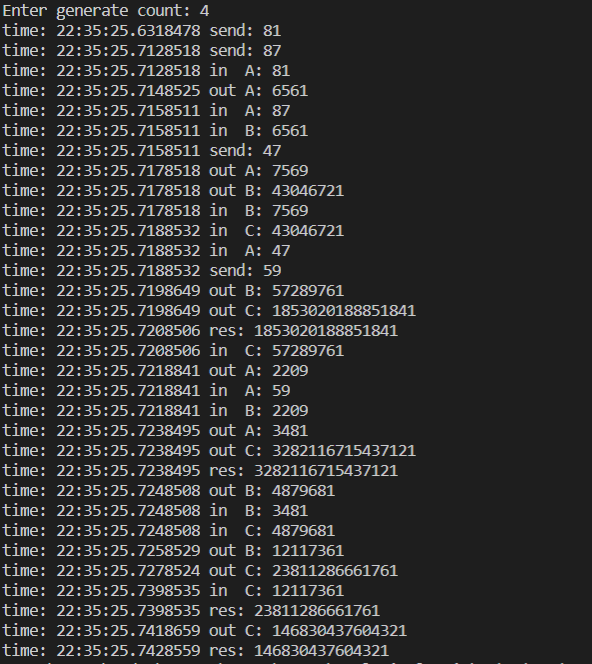
\includegraphics[scale=0.9]{testing.png}
            \caption{Результаты тестирования алгоритмов.}
            \label{png:testing:result}
        \end{figure}
\newpage
\chapter{Экспериментальный раздел}
\label{cha:research}
    В данном разделе будут проведены эксперименты для проведения 
    сравнительного анализа на основе замеров времени работы алгоритмов.

    \section{Сравнительный анализ на основе замеров времени работы алгоритмов}
        В рамках данной работы были проведёны следующие эксперименты по вычислению: 
        \begin{enumerate}
            \item времени работы системы в линейной и конвейерной реализациях (график \ref{graph:test:models});
        \end{enumerate}

        Тестирование проводилось на ноутбуке с процессором
        Intel(R) Core(TM) i5-7200U CPU 2.50 GHz \cite{processor-i5-7200u}
        под управлением Windows 10 с 8 Гб оперативной памяти.

        В ходе экспериментов по замеру времени работы в линейной и конвейерной реализациях было установлено,
        что конвейерная модель обрабатывает элементы в $ \approx 2.6 $ раза
        быстрее, чем линейная. Это объясняется тем,
        что одновременно обработываются разные элементы на разных этапах.
        
        По результатам исследования зависимости времени работы конвейерной системы от времени работы этапа  
        можно сделать вывод, что если одна из стадий намного более трудоемкая, чем остальные,
        то конвейерная обработка становится неэффективной,
        так как производительность всей программы будет упираться в производительность этой стадии,
        и разница между обычной обработкой и конвейерной будет малозаметна.
        В таком случае можно либо разбить трудоемкую стадию на набор менее трудоемких,
        либо выбрать другой алгоритм, либо отказаться от конвейерной обработки.


    \begin{figure}[h!]
        \centering
        \begin{tikzpicture}
            \begin{axis}[
                legend pos = north west,
                grid = major,
                xlabel = Количество элементов,
                ylabel = {Время, мс},
                height = 0.5\paperheight, 
                width = 0.75\paperwidth
            ]
            
            \addplot table[x=n, y=linear] {data/time-models.dat};
            \addplot table[x=n, y=conveyor] {data/time-models.dat};
            \legend{
                Линейная,
                Конвейерная
            };
            \end{axis}
        \end{tikzpicture}
        \caption{График зависимости времени работы от модели системы} 
        \label{graph:test:models}
    \end{figure}


\newpage

\backmatter % Здесь заканчивается нумерованная часть документа и начинаются ссылки и
\Conclusion
    В ходе выполнения данной лабораторной работы был изучен
    муравьиный алгоритм и приобретены навыки параметризации
    методов на его примере. 
    Реализованы следующие задачи:
    \begin{itemize}
        \item реализованы два алгоритма решения задачи коммивояжера;
        \item замерено время выполнения алгоритмов;
        \item проведено исследование уравьиного алгоритма от параметров.
    \end{itemize}
    
    Использовать муравьиный алгоритм для решения задачи коммивояжера выгодно (с точки зрения времени выполнения),
    в сравнении с алгоритмом полного перебора, в случае если в анализируемом графе вершин больше либо равно 9.
    Так, например, при размере графа 11, муравьиный алгоритм работает быстрее чем алгоритм полного перебора в 900 раз.
    Стоит отметить, что муравьиный алгоритм не гарантирует что найденный путь будем оптимальным,
    так как он является эвристическим алгоритмом, в отличии от алгоритма полного перебора.
    
\bibliographystyle{gost780u}
\bibliography{report}

	\addcontentsline{toc}{section}{Список литературы}
	
	\begin{center}
	\begin{thebibliography}{3}
	\bibitem{binary-search}
	IDE Visual Studio 2019. Режим доступа: (дата обращения: 11.09.2020) Свободный. URL: https://visualstudio.microsoft.com/ru/vs/
	\bibitem{c-sharp}
	Python. Режим доступа: (дата обращения: 01.10.2020) Свободный. URL: https://www.python.org/
	\bibitem{vs}
	Go [Электронный ресурс]. Режим доступа: (дата обращения: 01.10.2020) Свободный. URL: https://golang.org/
	\bibitem{proc}
	Intel® Core™ i5-8250U Processor [Электронный ресурс]. Режим доступа: (дата обращения: 26.09.2020) Свободный. URL: https://www.intel.com/content/www/us/en/products/processors/core/i5-processors/i5-8250u.html
	\bibitem{parll1}
	Синхронизация потоков. Проблема производителя и потребителя. [Электронный ресурс]. Режим доступа: (дата обращения: 28.11.2020) Свободный. URL: https://moodle.kstu.ru/mod/page/view.php?id=9274
	\bibitem{parll2}
	Типовые модели параллельных приложений [Электронный ресурс]. Режим доступа: (дата обращения: 28.11.2020) Свободный. URL: https://intuit.ru/studies/courses/5938/1074/lecture/16465?page=3

	\end{thebibliography}
	\end{center}

\end{document}